\section{Experiments}
\label{sec:experiments}
% add data description
I applied the proposed framework on real world dynamic data.
This section will provide implementation details and parameter settings, and will also provide results and observations from experiments.

\subsection{Landmark detection results}
\label{sec:landmark_detection_results}
First I conducted a preliminary experiment before further developing landmark detection techniques by answering the question: How would landmark dynamics affect final airway analysis?

I studied this on the first dynamic data I got from our collaborator.
The subject was 59 days old and only had a TC annotation \footnote{The other annotation nearest TC was TVC, and it was not visible due to the doctor's choice of scan area}. 
I then chose the top of the airway as a dummy landmark TVC and the TC for registration.
I manually annotated the these two landmarks in each frame and computed the Euclidean difference between landmarks with respect to time.

Figure~\ref{fig:landmark_dynamics} shows the movement of landmarks between each frame in millimeter.
In this figure, TC shows a significant changes after time step 4.
The landmark dynamics revealed that the airway of the subject was changing a lot in a period of time.
%This observation matched our measurement of cross-sectional areas.

Figure~\ref{fig:landmark_updated} shows the results of the airway measurement of the 59 days old subject.
The difference between the left and right results in Figure~\ref{fig:landmark_updated} is whether considering the landmark dynamics.
The left result shows eight functional curves registered with the same TC and TVC annotation at the first frame.
The right result shows eight functional curves registered with the updated TC and TVC annotations at each frame.
We can see that Figure~\ref{fig:landmark_updated} (right) captured a cross-sectional area drop in the end of the functional data.
Figure~\ref{fig:landmark_updated} (left), however, lost this feature (compare the green curves on the left and on the right.)
Because an area drop is a critical feature for airway analysis, I considered updating landmarks in each time frame is an important issue and further developed the framework described in Section~\ref{sec:landmark_detection}.

\begin{figure}[tb]
  \begin{center}
    \begin{tabular}{ccc}
    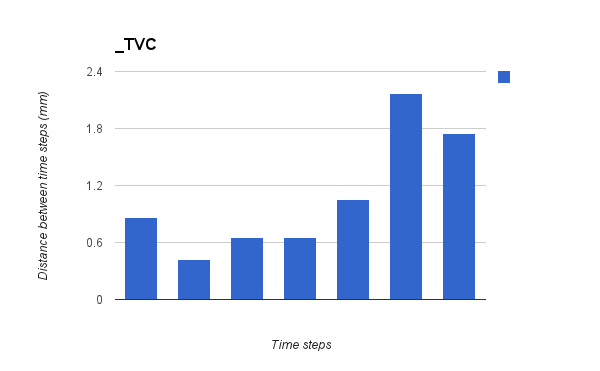
\includegraphics[width=\figwidth] {fig/d_TVC.png}
    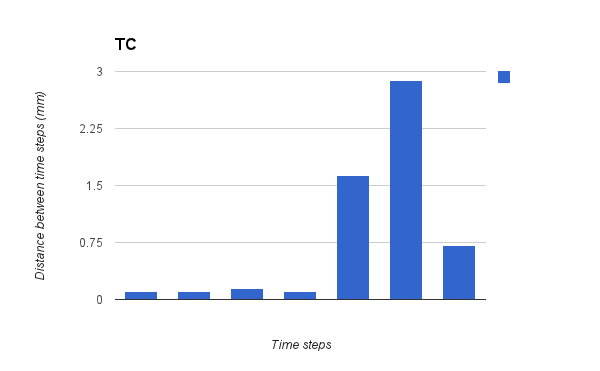
\includegraphics[width=\figwidth] {fig/dTC.png}
    \end{tabular}
    \caption{ \label{fig:landmark_dynamics} Visualization of the landmark dynamics of a 59 days subject. 
    }
  \end{center}
\end{figure}

\begin{figure}[tb]
  \begin{center}
    \begin{tabular}{ccc}
    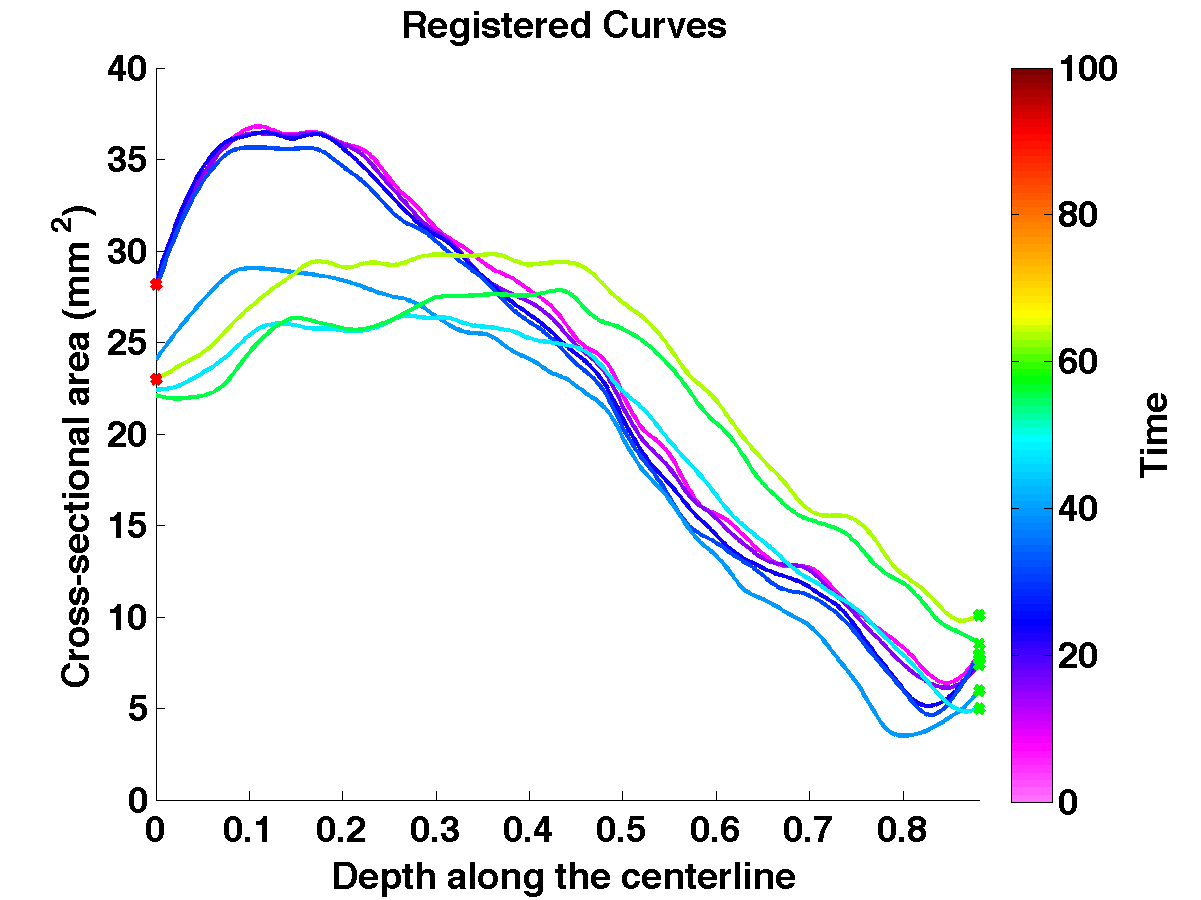
\includegraphics[width=\figwidth] {fig/registered_1_updates_0.png}
    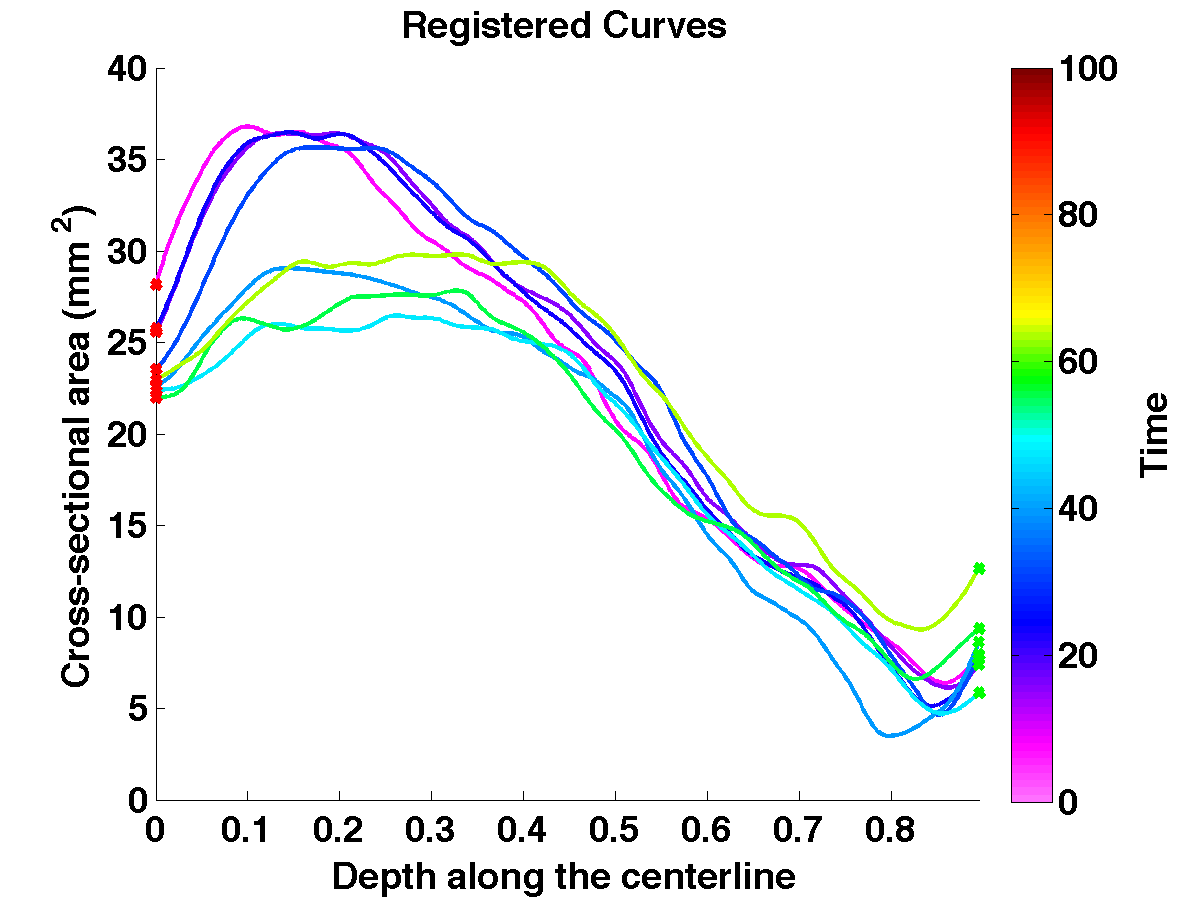
\includegraphics[width=\figwidth] {fig/registered_1_updates_1.png}
    \end{tabular}
    \caption{ \label{fig:landmark_updated} Cross-sectional area of a 59 days old subject with different registration landmarks. {\bf Left.} The result using the same landmarks for each time step. {\bf Right.} The result with updated landmarks for each time step. Note that in the end of functional data, a lower cross-sectional measurement disappeared on the left but remains on the right.
    }
  \end{center}
\end{figure}

Since updating landmarks with the subject's deformation is need, I applied the automatically landmark detector described in Section~\ref{sec:methods}.
The detector has training stage and detection stage.

{\bf Training.} 
The training set had 95 3D CT images with manually annotated landmarks from nasal spine, choana, epiglottis tip, TVC, and TC.
I trained a linear SVM classifier for TC using CHOG features.
Each subject provided a positive example which would be HOG features extracted from three orthogonal bounding boxes passing through the landmark TC.
The scale of the bounding boxes was chosen as twice of the minimum rectangle covering the airway in the axial plane.
The negative examples were drawn at an uniform distributed scale and location that did not intersect with the positive bounding boxes.
For each positive example, I drawn ten times negative samples.

{\bf Detection.}
For a 512x512x640 3D CT image, there are too many possible hypotheses of scale and location.
I utilized a prior of geometry to eliminate possible hypotheses.
Once we have the segmentation of the image, we only look at the segmented trachea for landmarks.
In each depth I only drew one hypothesis from the center of the airway using the scale with the same heuristic in training.
The trained SVM classifier predicted a score of the landmark likelihood given different depth.
Figure~\ref{fig:landmark_detection} illustrated the likelihood prediction on training data.
We can see there are some outliers in prediction on the training data.
Due to these outliers, the mean prediction error was 24.7436 (mm) and the standard deviation was 29.4251 (mm).

\begin{figure}[tb]
  \begin{center}
    \begin{tabular}{ccc}
    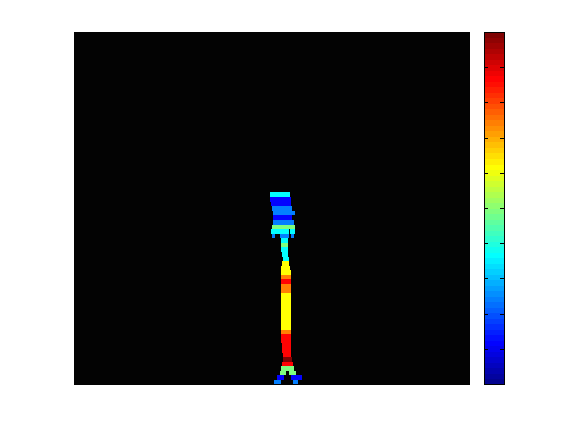
\includegraphics[width=\figwidth] {fig/CRL02_TracheaCarina_left.png}
    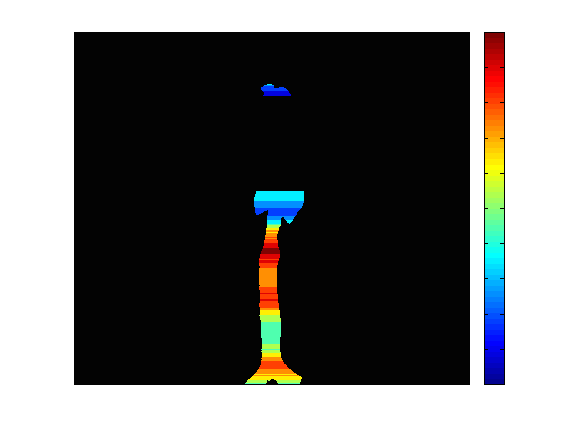
\includegraphics[width=\figwidth] {fig/CRL04_TracheaCarina_left.png}
    \end{tabular}
    \caption{ \label{fig:landmark_detection} Illustration of the likelihood of landmark TC. {\bf Left.} In most cases the detector located TC in a correct position. {\bf Right.} Even failure cases show the correct TC position as their second or third choice.
    }
  \end{center}
\end{figure}


\begin{table}
  \centering
   \caption{Errors of landmark prediction methods of a 134 month subject (Fleck-005).
   }
  \begin{tabular}{r || cccc}
  & mean (mm) & std. (mm) & mean (px) & std. (px) \\
  \hline
  None & 4.7575 & 2.5314 & 18.6614 & 10.2052 \\
  CHOG & 2.8812 & 1.6134 & 9.3357 & 6.6279 \\
  \end{tabular}
  \label{tab:landmarks}
\end{table}


Now let us try to apply the detector on dynamic data and see if it can handle landmark dynamics.
I applied the detector on a 134 month old subject (Fleck-005).
Table~\ref{tab:landmarks} summarized the errors of landmark prediction on TC for when landmark dynamics are not considered, and my landmark detector using CHOG\footnote{One outlier is removed. Count the outlier than the mean would be 3.9280 mm (12.7448 px) and the std. would be 4.4680 mm (15.0649 px).}.
My automatic landmark detector reduced the errors of the mean and standard deviation.
However, the problem of outliers reminded for one frame.

% \begin{figure}[tb]
%   \begin{center}
%     \begin{tabular}{ccc}
%     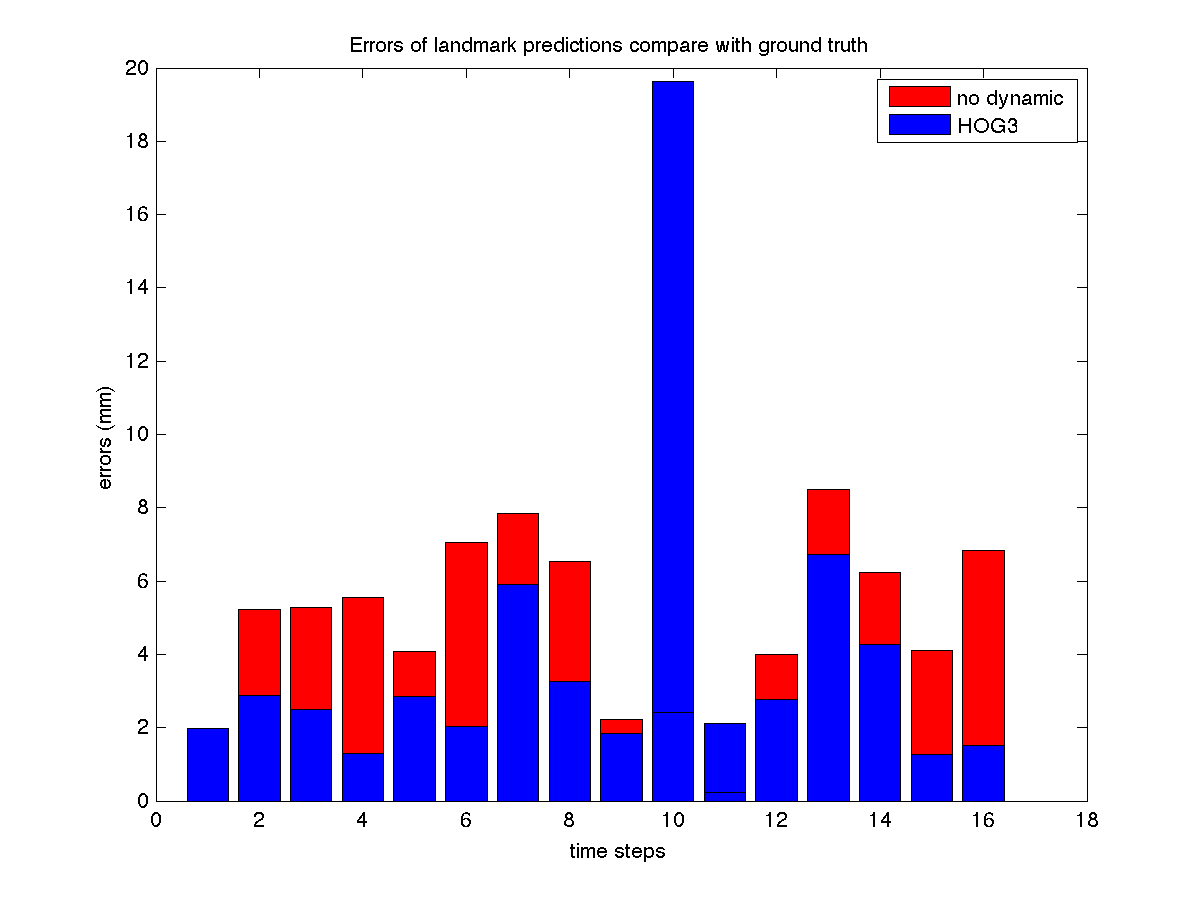
\includegraphics[width=0.4\linewidth] {fig/landmark_errors.png}
%     \end{tabular}
%     \caption{ \label{fig:landmark_errors} Illustration of the landmark prediction errors in each time step for subject Fleck-005. Red bar shows the errors of neglecting landmark dynamics and blue bar shows the errors from the proposed algorithm. Note that there is an outlier in time step 10.
%     }
%   \end{center}
% \end{figure}

\subsection{Dynamic airway analysis}
\label{sec:dynamic_airway_analysis}
\begin{figure}[tb]
  \begin{center}
    \begin{tabular}{ccc}
    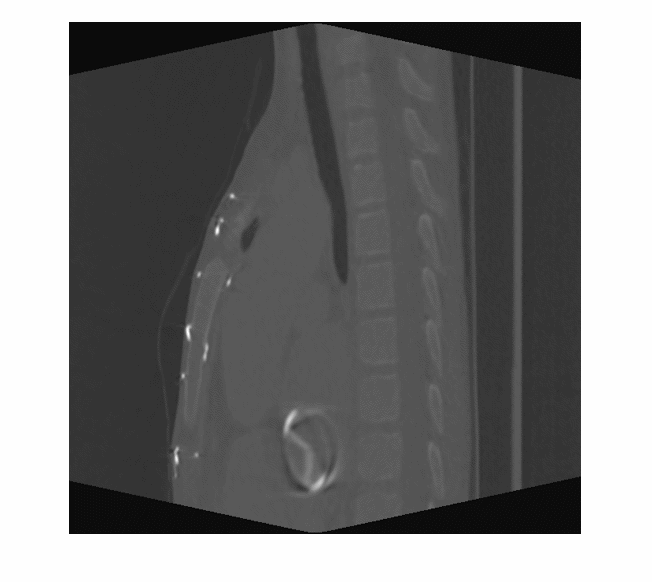
\includegraphics[height=\figheight] {fig/Fleck_007.png}
    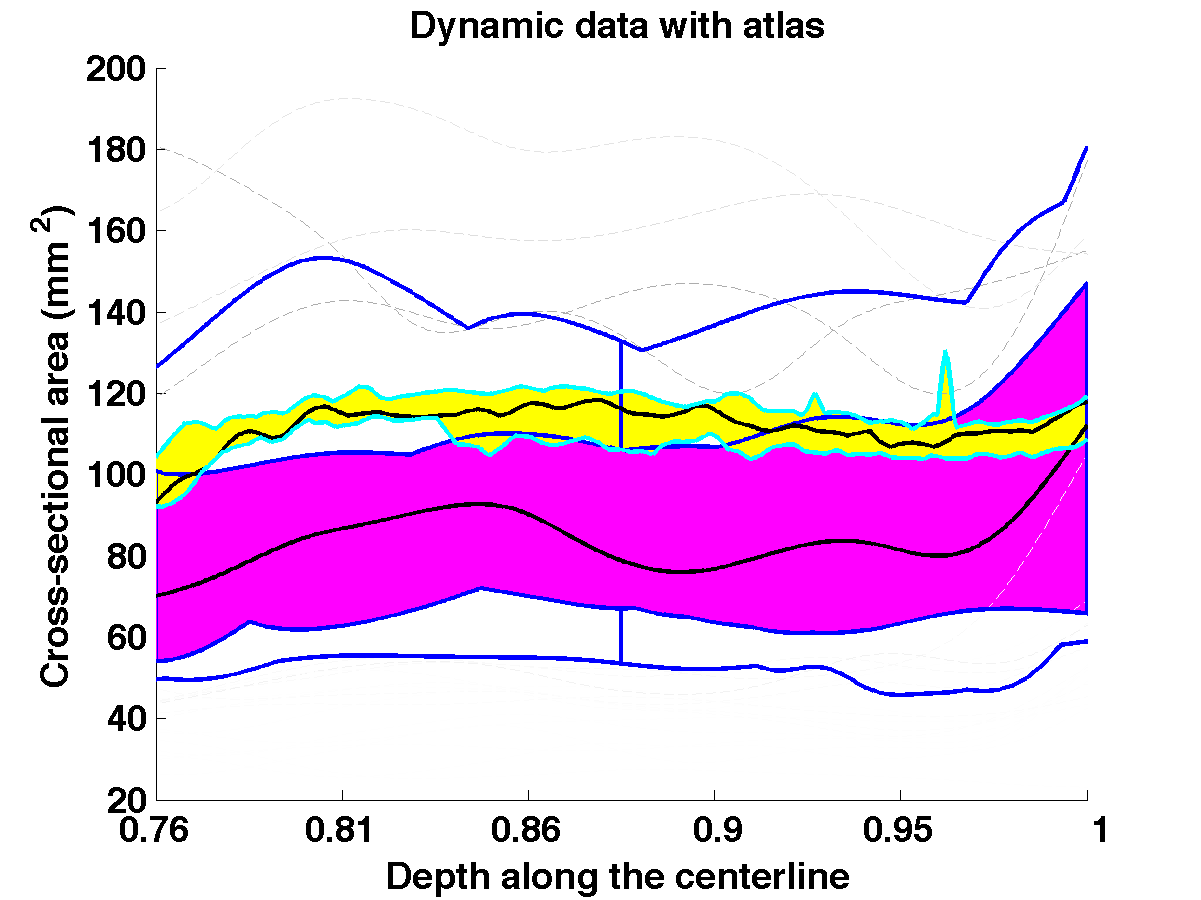
\includegraphics[width=\figwidth] {fig/Fleck_007_wfbplot.png} \\
    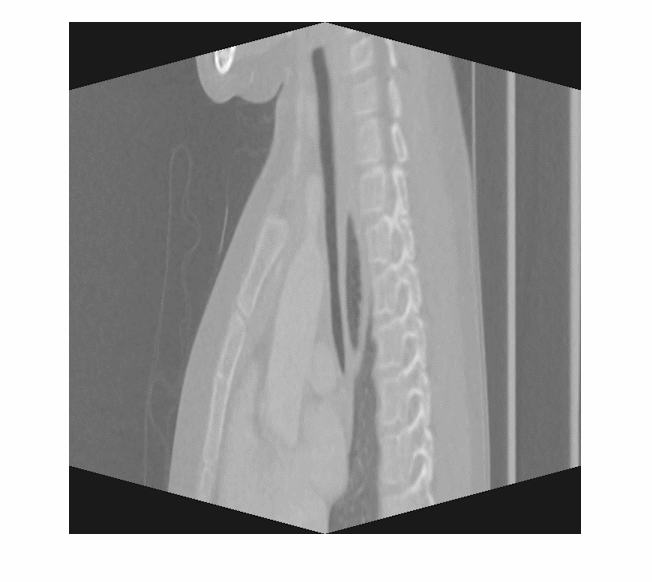
\includegraphics[height=\figheight] {fig/Fleck_008.png}
    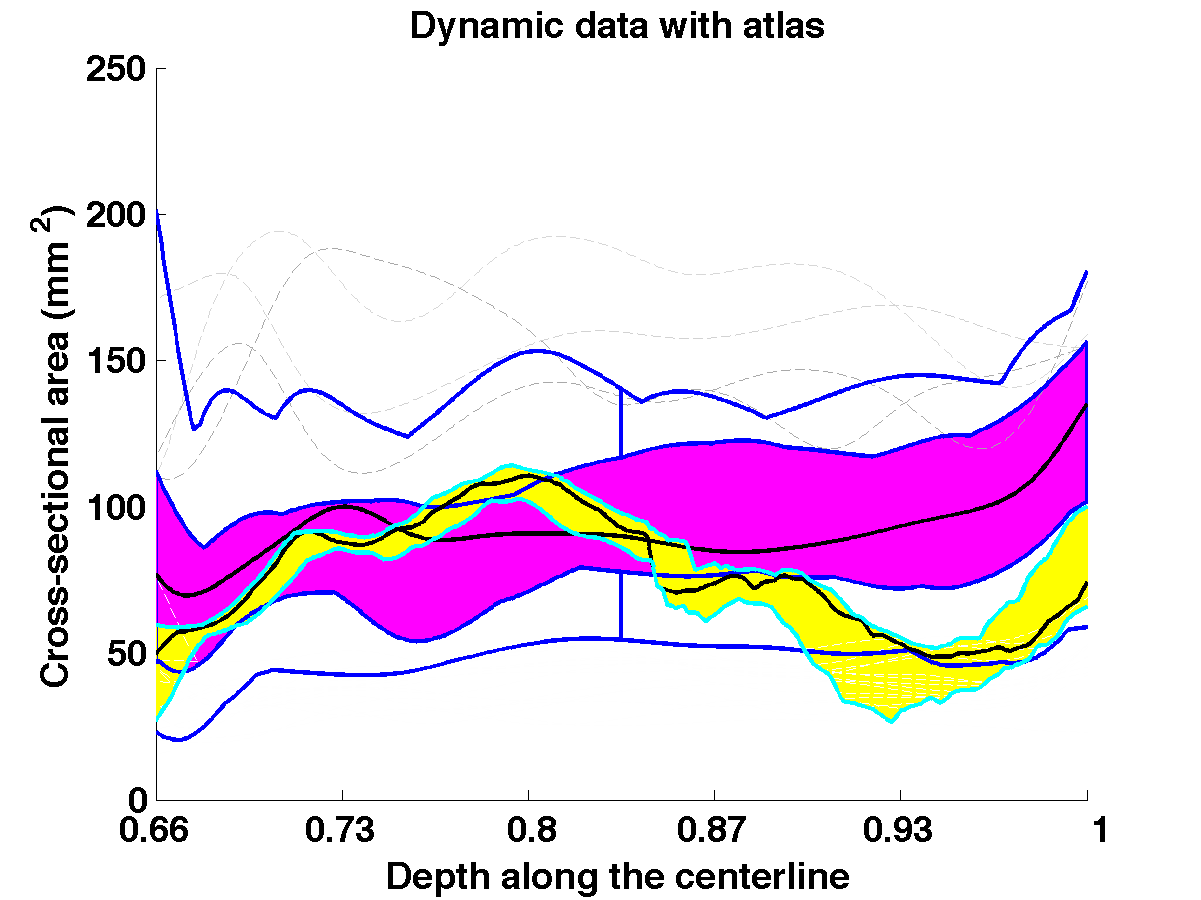
\includegraphics[width=\figwidth] {fig/Fleck_008_wfbplot.png} \\
    \end{tabular}
    \caption{ \label{fig:Fleck} Dynamic airway atlas for subject Fleck-007 and Fleck-008. {\bf Left.} A slice of dynamic data. {\bf Right.} The purple area is the interquartile range of the age-adapted normal control atlas. The blue curves are the maximum and the minimum of the normal control atlas. The yellow area is the entire estimation range of the dynamic subject over the different time steps. The depth is in a unified scale, where 0.66 is TVC and 1 is TC.
    }
  \end{center}
\end{figure}
I performed dynamic airway analysis using functional boxplots on real data provided by a physician.
The normal control atlas was built from 68 healthy subjects in control group using the method in~\cite{hong2014statistical}.
Figure~\ref{fig:Fleck} shows the results.
Here I compared these results with the comments from the doctor for two cases.

{\bf Fleck-007, 114 months.}
The subject seemed to have a narrow airway on the CT scan at the first glance.
However, comparing with the normal control atlas, this subject definitely had an airway size larger than average normal control data.
Also, the doctor's comment was ``No significant change in the trachea or bronchi during cough maneuver. No evidence of tracheobronchomalacia.'', which qualitatively agrees with the analysis result.

{\bf Fleck-008, 129.6 months.}
For this subject the airway seemed normal in one slice.
Yet it was considered narrowed compared with the normal control atlas, and it had large dynamics especially from the depth 0.87 to 1.
The depth 0.66 means TVC and 1 means TC.
So the subject had narrowed trachea near TC.
Quote the doctor's comment ``Dynamic, 2.5 cm long narrowing of the mid to distal thoracic trachea caused by the adjacent left-sided aortic arch. The luminal diameter of the trachea changes from 11 mm during diastole to 5 mm in systole'', the subject did show problems in the mid to distal thoracic trachea, the analysis results qualitatively agree with the observation.